\begin{appendices}
\chapter{Multi layer perceptron (First MLP) charts}
\begin{figure}[hbtp]

\centering
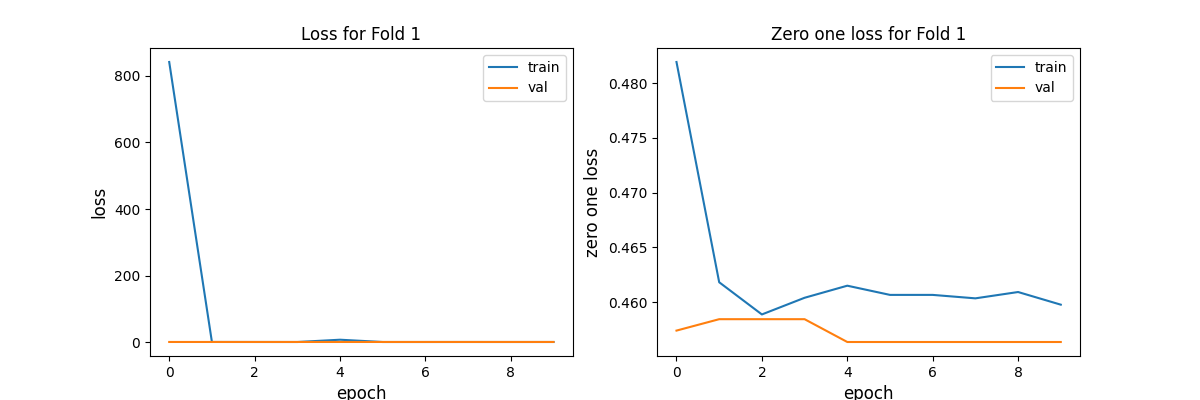
\includegraphics[scale=0.5]{../Images/mlp01_fold_1_zeroplot.png}
\end{figure}
\begin{figure}[hbtp]

\centering
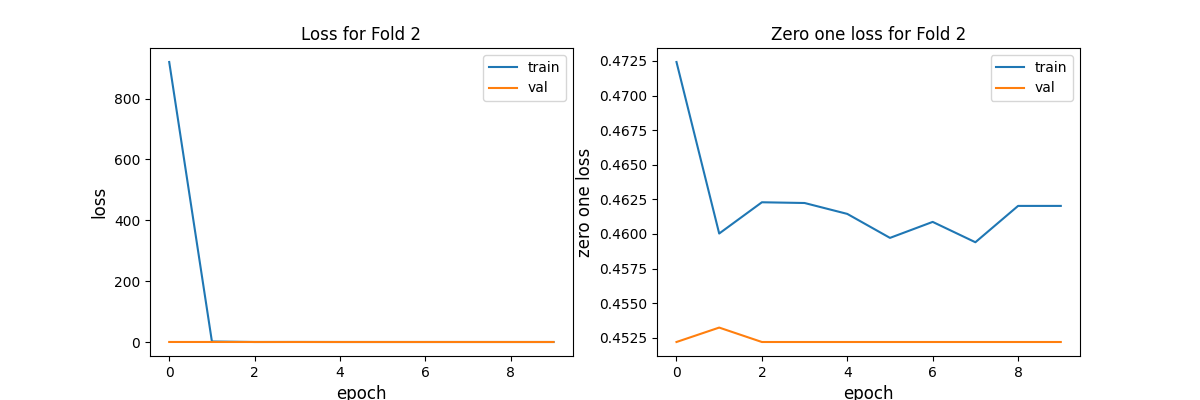
\includegraphics[scale=0.5]{../Images/mlp01_fold_2_zeroplot.png}
\end{figure}
\begin{figure}[hbtp]

\centering
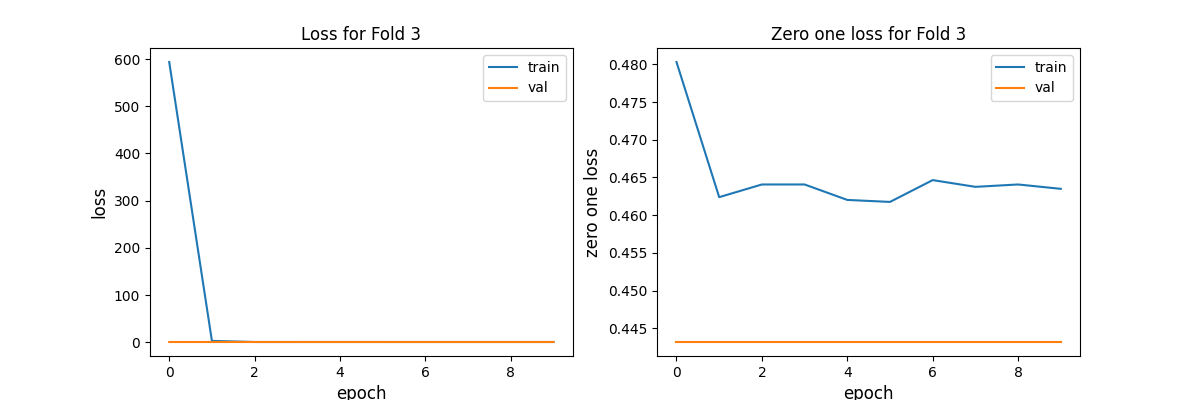
\includegraphics[scale=0.5]{../Images/mlp01_fold_3_zeroplot.png}
\end{figure}
\begin{figure}[hbtp]

\centering
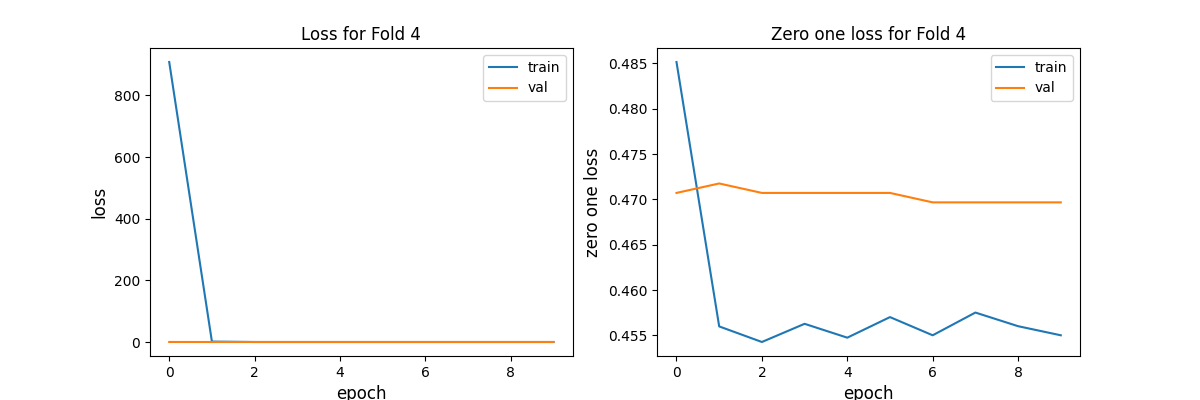
\includegraphics[scale=0.5]{../Images/mlp01_fold_4_zeroplot.png}
\end{figure}
\begin{figure}[hbtp]

\centering
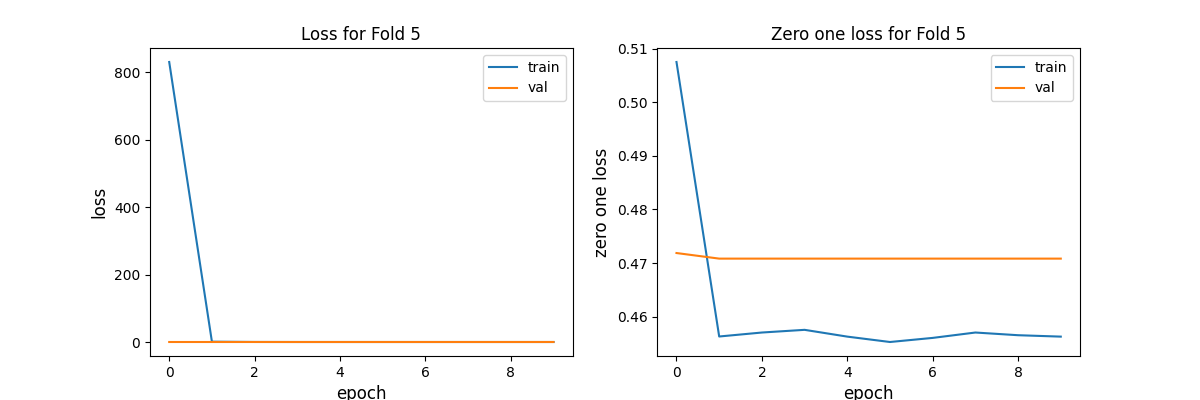
\includegraphics[scale=0.5]{../Images/mlp01_fold_5_zeroplot.png}
\end{figure}
\chapter{Multi layer perceptron (First MLP after hypertuning) charts}
\begin{figure}[hbtp]

\centering
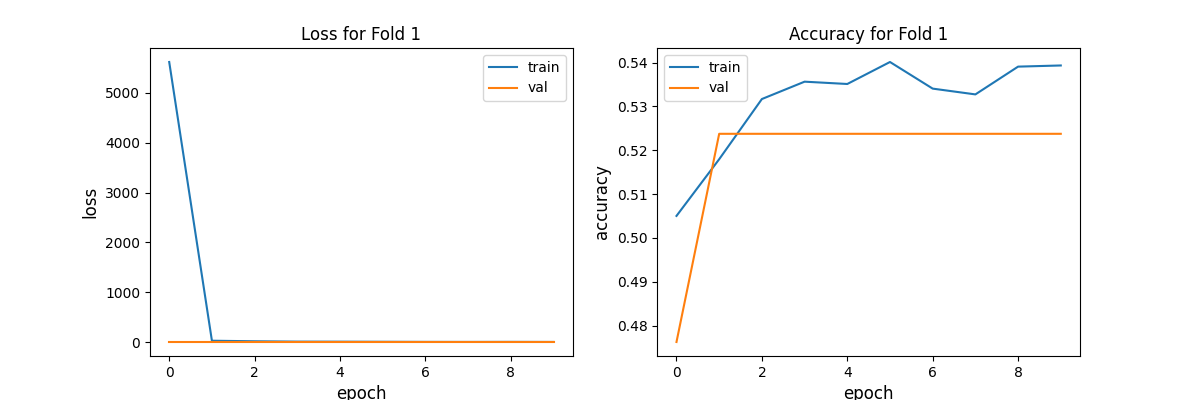
\includegraphics[scale=0.5]{../Images/mlp02_fold_1_plot.png}
\end{figure}
\begin{figure}[hbtp]

\centering
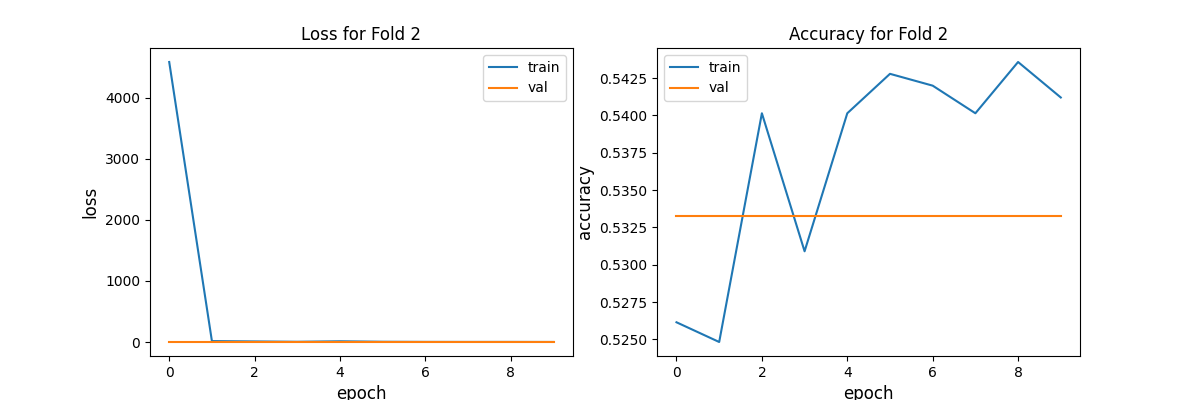
\includegraphics[scale=0.5]{../Images/mlp02_fold_2_plot.png}
\end{figure}
\begin{figure}[hbtp]

\centering
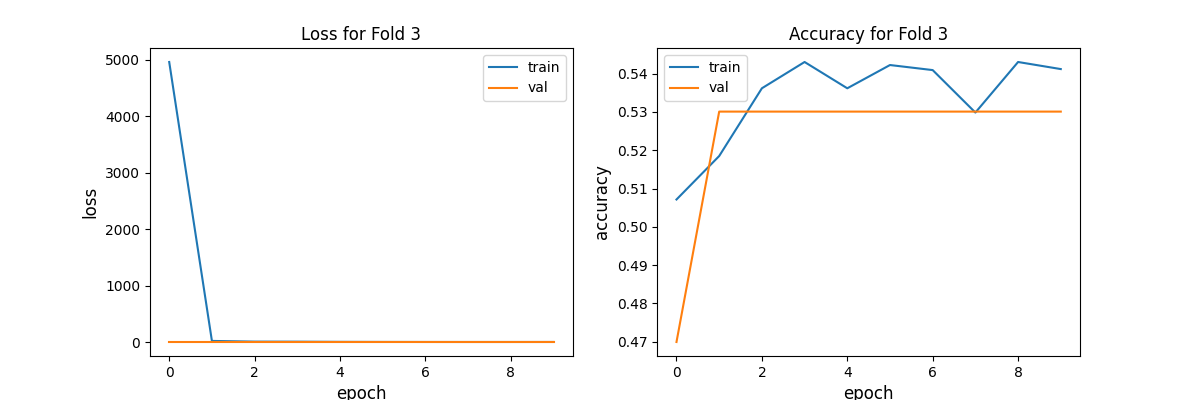
\includegraphics[scale=0.5]{../Images/mlp02_fold_3_plot.png}
\end{figure}
\begin{figure}[hbtp]

\centering
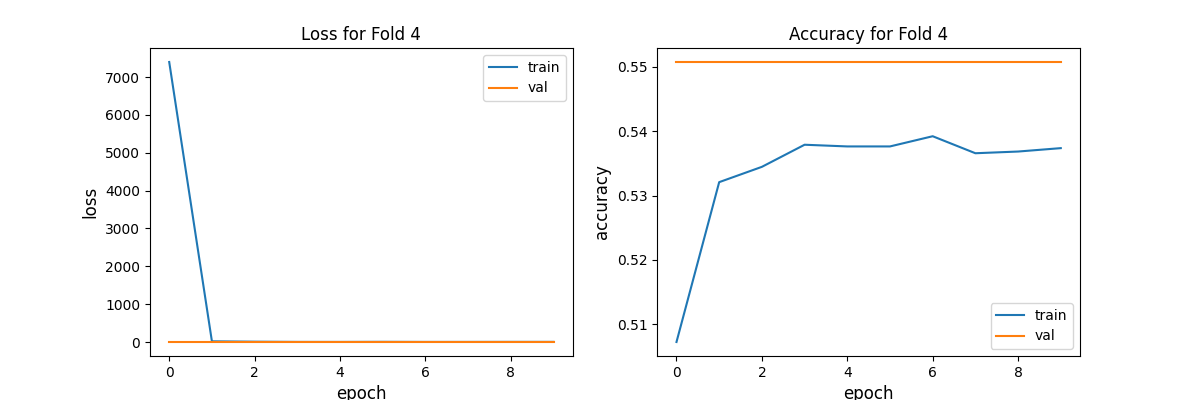
\includegraphics[scale=0.5]{../Images/mlp02_fold_4_plot.png}
\end{figure}
\begin{figure}[hbtp]

\centering
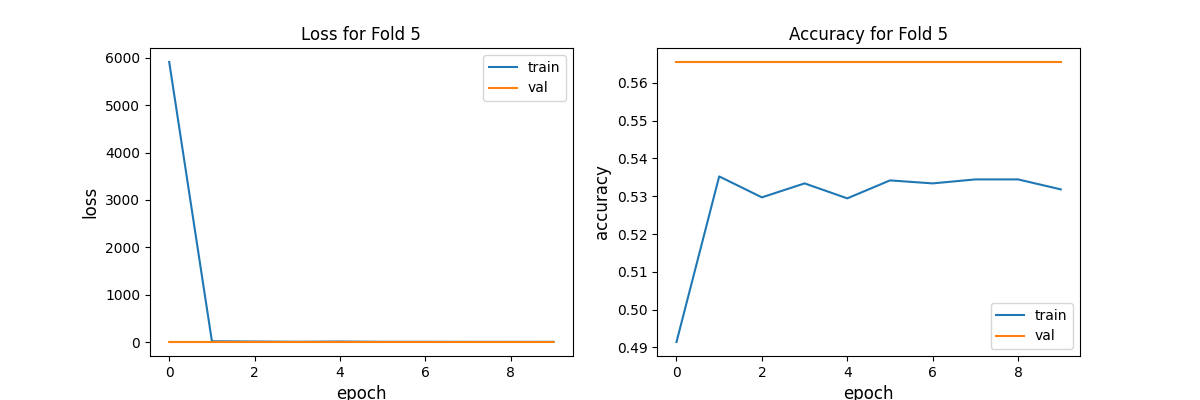
\includegraphics[scale=0.5]{../Images/mlp02_fold_5_plot.png}
\end{figure}
\begin{figure}[hbtp]

\centering
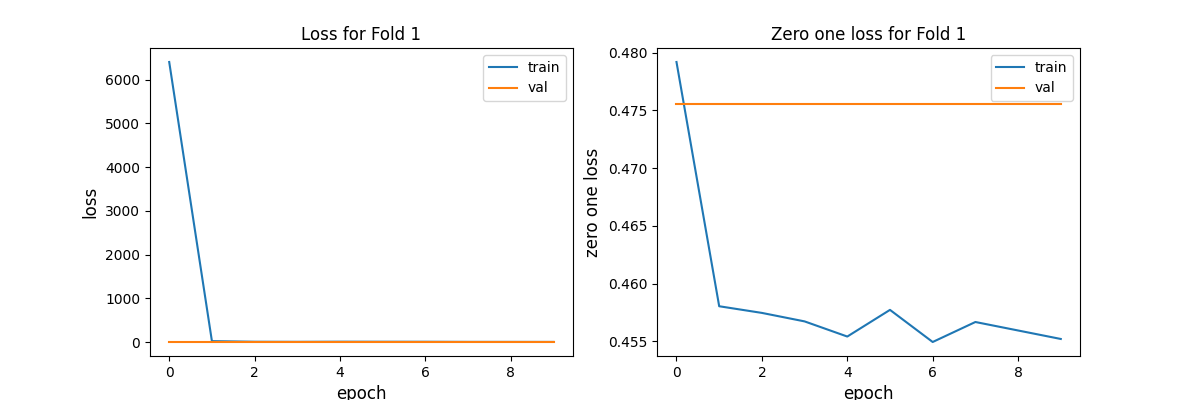
\includegraphics[scale=0.5]{../Images/mlp02_fold_1_zeroplot.png}
\end{figure}
\begin{figure}[hbtp]

\centering
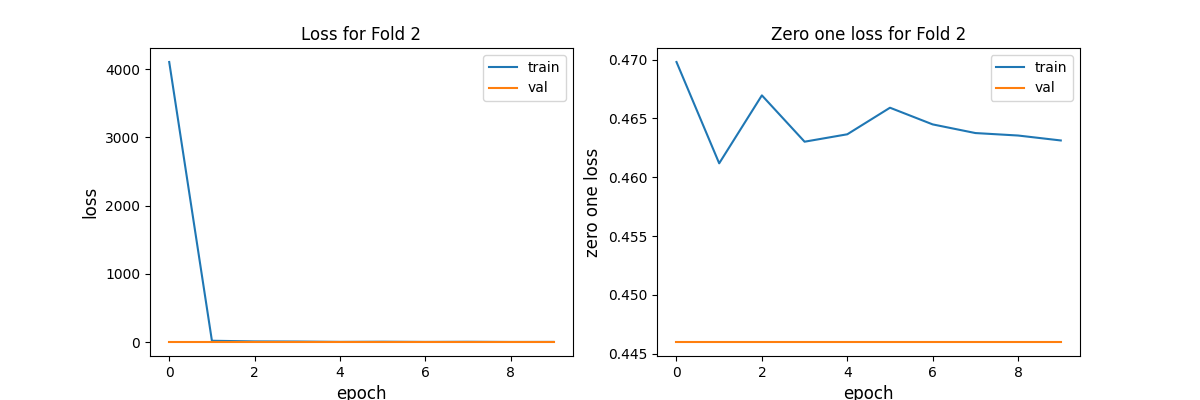
\includegraphics[scale=0.5]{../Images/mlp02_fold_2_zeroplot.png}
\end{figure}
\begin{figure}[hbtp]

\centering
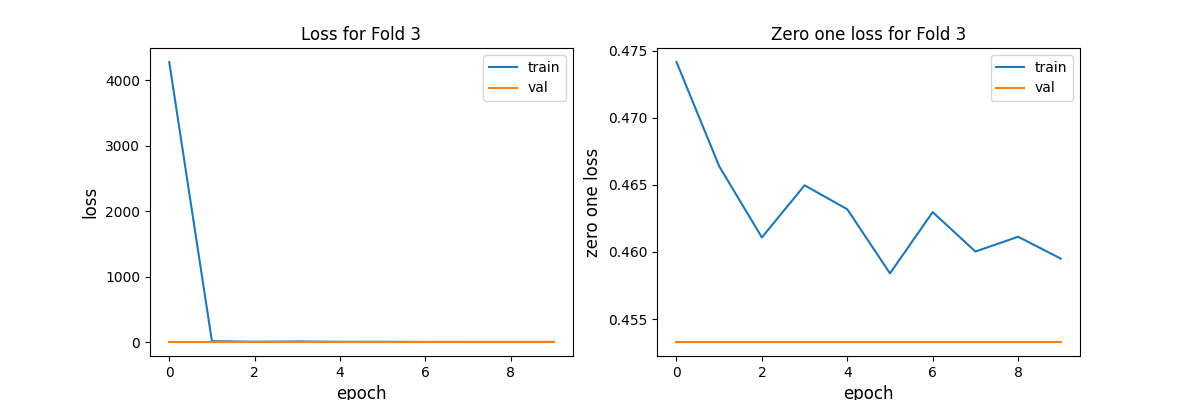
\includegraphics[scale=0.5]{../Images/mlp02_fold_3_zeroplot.png}
\end{figure}
\begin{figure}[hbtp]

\centering
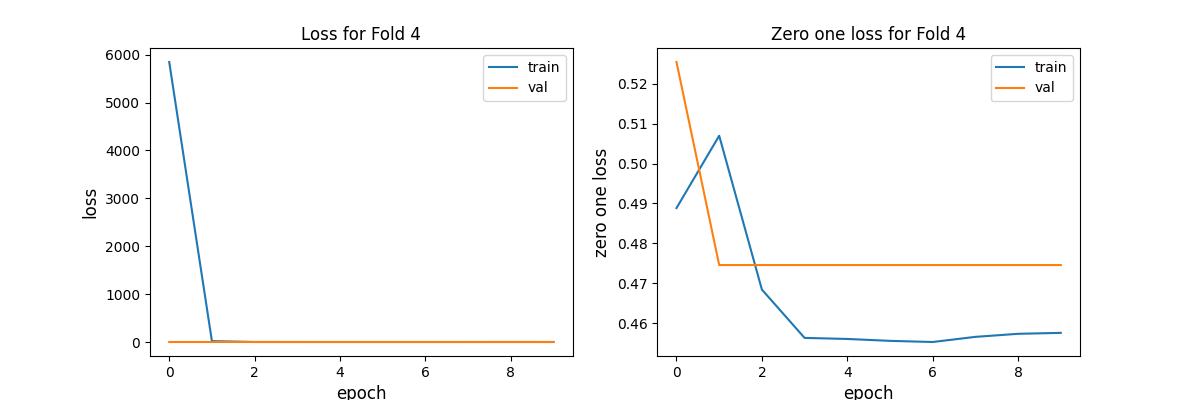
\includegraphics[scale=0.5]{../Images/mlp02_fold_4_zeroplot.png}
\end{figure}
\begin{figure}[hbtp]

\centering
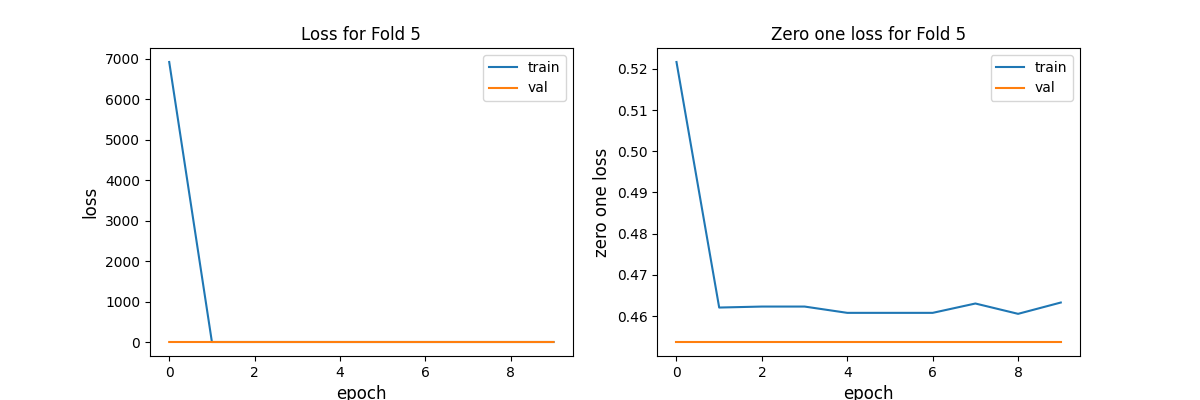
\includegraphics[scale=0.5]{../Images/mlp02_fold_5_zeroplot.png}
\end{figure}
\chapter{Convolutional Neural Network (CNN) charts}
\begin{figure}[hbtp]

\centering
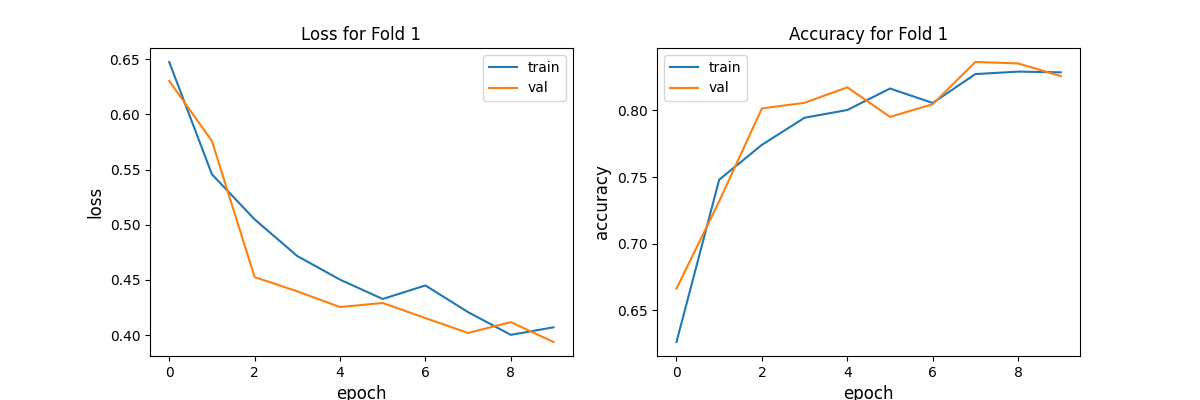
\includegraphics[scale=0.5]{../Images/cnn01_fold_1_plot.png}
\end{figure}
\begin{figure}[hbtp]

\centering
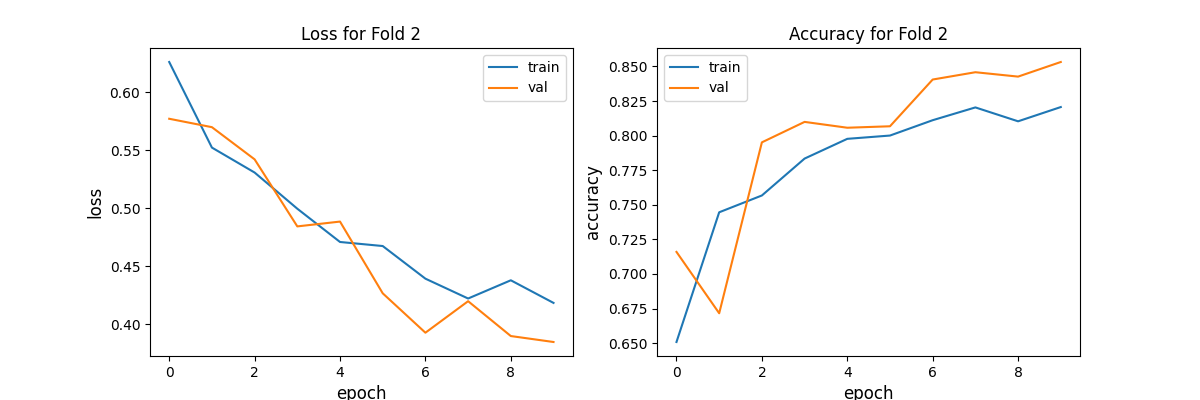
\includegraphics[scale=0.5]{../Images/cnn01_fold_2_plot.png}
\end{figure}
\begin{figure}[hbtp]

\centering
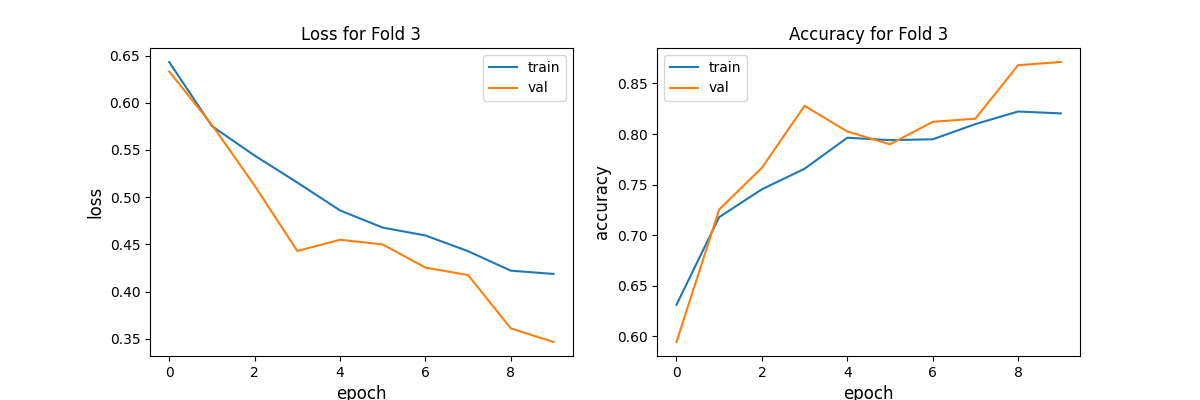
\includegraphics[scale=0.5]{../Images/cnn01_fold_3_plot.png}
\end{figure}
\begin{figure}[hbtp]

\centering
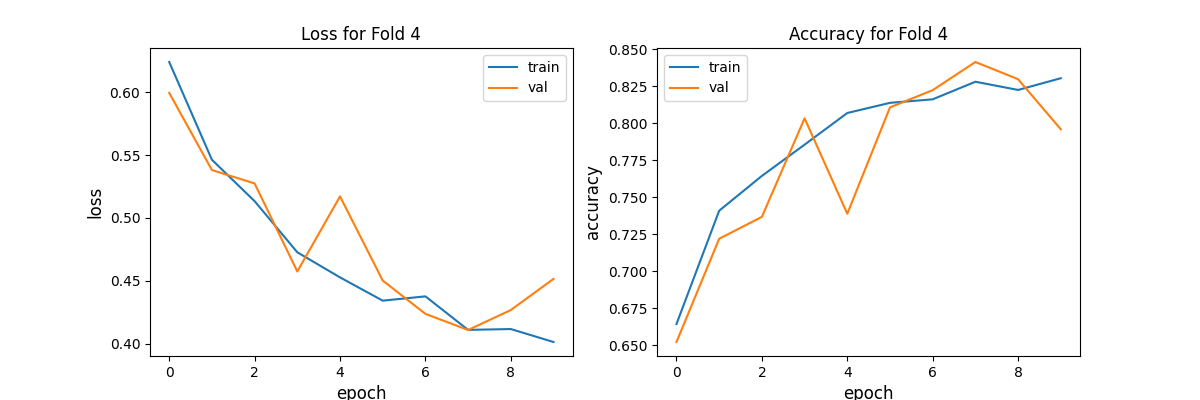
\includegraphics[scale=0.5]{../Images/cnn01_fold_4_plot.png}
\end{figure}
\begin{figure}[hbtp]

\centering
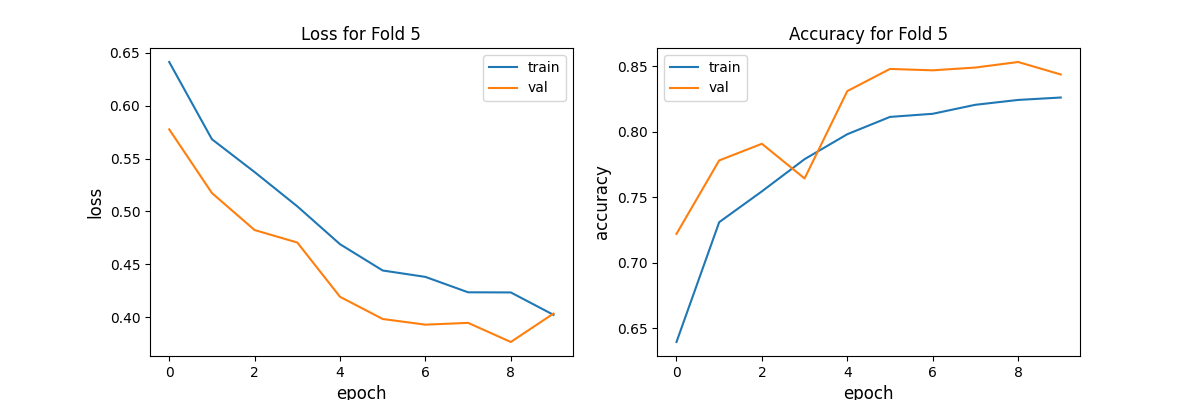
\includegraphics[scale=0.5]{../Images/cnn01_fold_5_plot.png}
\end{figure}
\begin{figure}[hbtp]

\centering
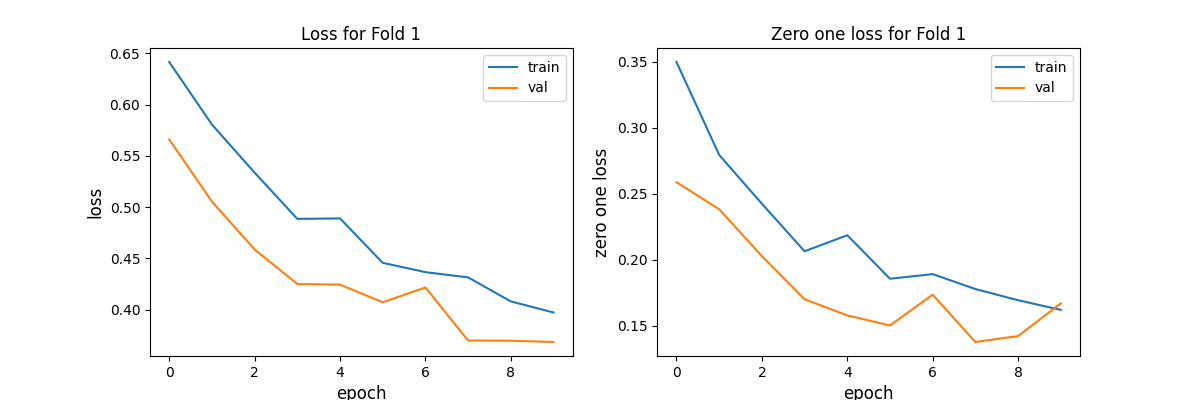
\includegraphics[scale=0.5]{../Images/cnn01_fold_1_zeroplot.png}
\end{figure}
\begin{figure}[hbtp]

\centering
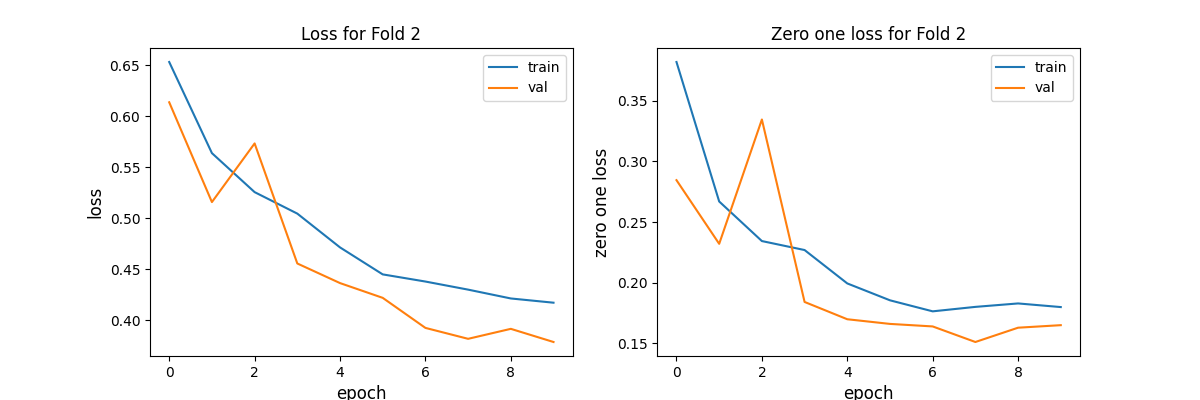
\includegraphics[scale=0.5]{../Images/cnn01_fold_2_zeroplot.png}
\end{figure}
\begin{figure}[hbtp]

\centering
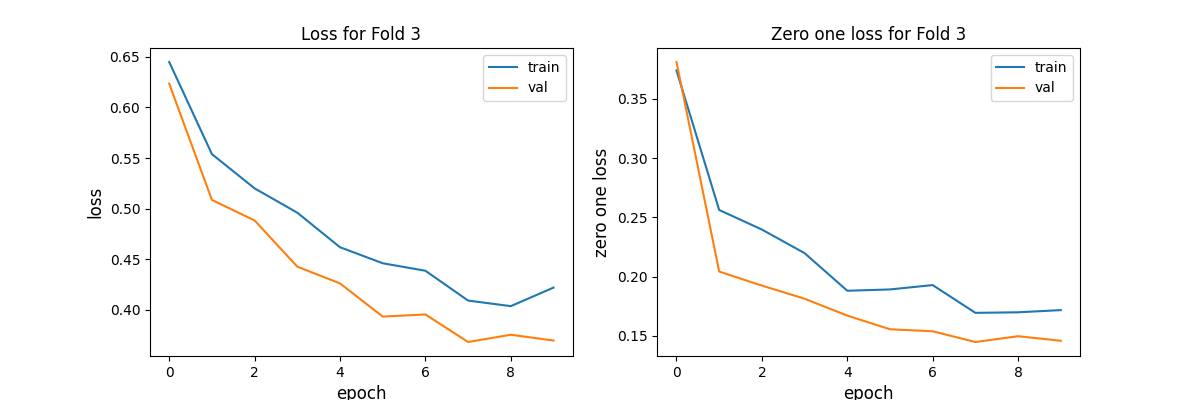
\includegraphics[scale=0.5]{../Images/cnn01_fold_3_zeroplot.png}
\end{figure}
\begin{figure}[hbtp]

\centering
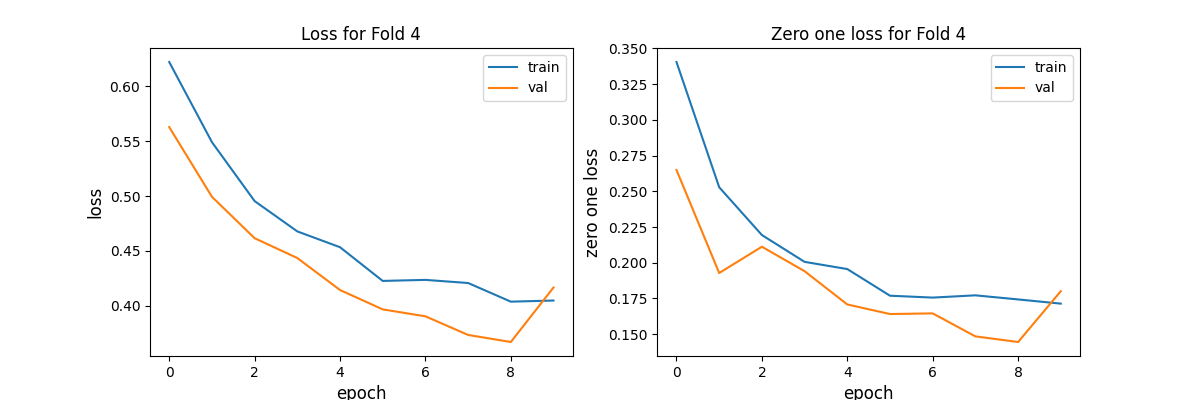
\includegraphics[scale=0.5]{../Images/cnn01_fold_4_zeroplot.png}
\end{figure}
\begin{figure}[hbtp]

\centering
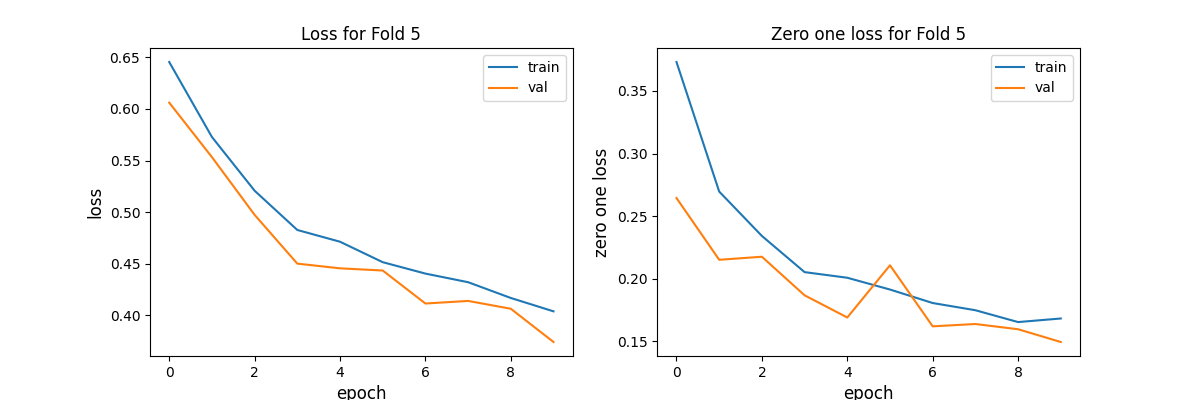
\includegraphics[scale=0.5]{../Images/cnn01_fold_5_zeroplot.png}
\end{figure}
\chapter{Deep Residual Learning (ResNet50) charts}
\begin{figure}[hbtp]

\centering
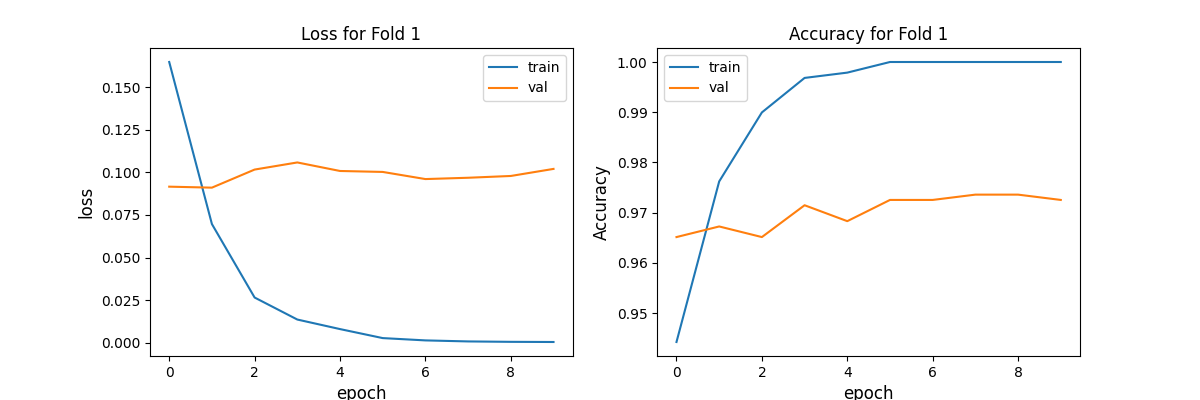
\includegraphics[scale=0.5]{../Images/res50_fold_1_plot.png}
\end{figure}
\begin{figure}[hbtp]

\centering
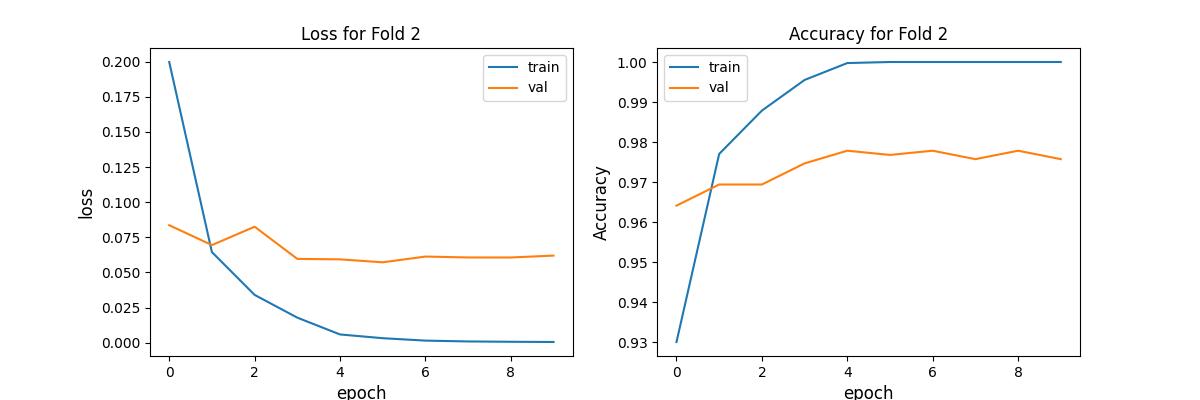
\includegraphics[scale=0.5]{../Images/res50_fold_2_plot.png}
\end{figure}
\begin{figure}[hbtp]

\centering
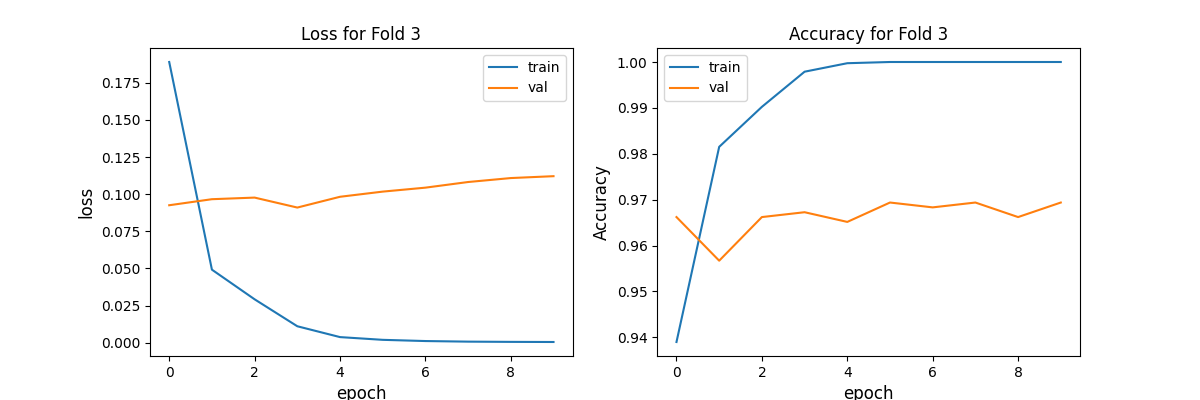
\includegraphics[scale=0.5]{../Images/res50_fold_3_plot.png}
\end{figure}
\begin{figure}[hbtp]

\centering
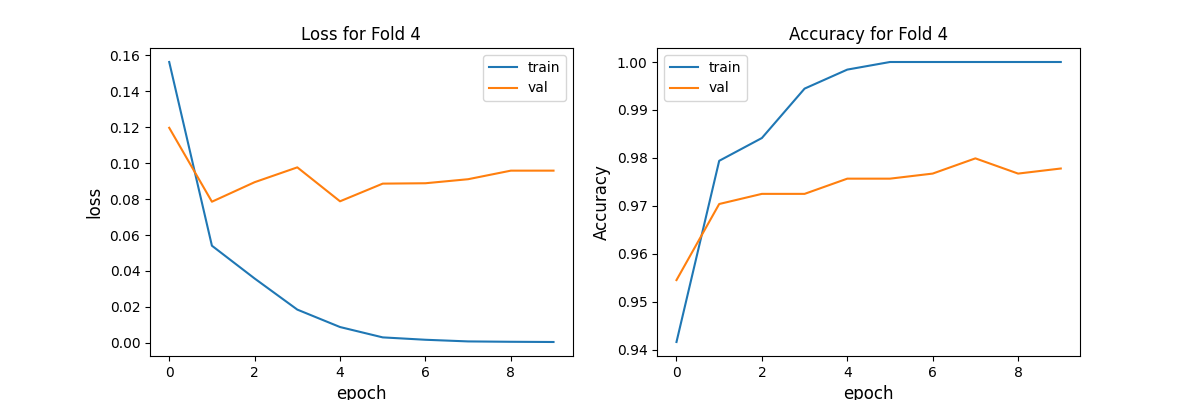
\includegraphics[scale=0.5]{../Images/res50_fold_4_plot.png}
\end{figure}
\begin{figure}[hbtp]

\centering
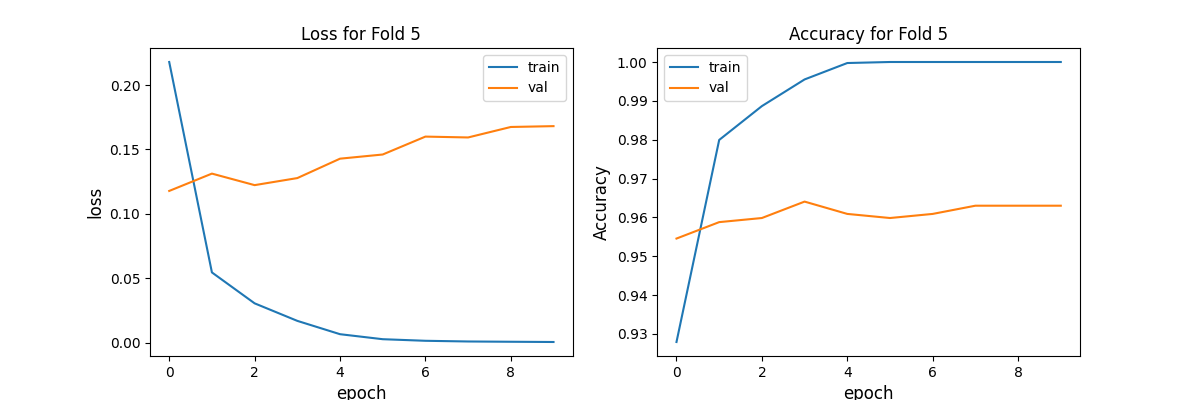
\includegraphics[scale=0.5]{../Images/res50_fold_5_plot.png}
\end{figure}

\end{appendices}